% Source: graduate-coursework/Research/How_to_write/00_Contrastive_Synthesis.tex
% Description: Historical emergence of major writing theories. Each theory arose largely as a corrective to the perceived failures of its predecessors, progressively widening the unit of analysis from the text to the full activity system.

\documentclass[border=4pt]{standalone}
\usepackage{newtxtext,newtxmath}
\usepackage{tikz}
\usetikzlibrary{arrows.meta,positioning,shapes.geometric,calc,decorations.pathreplacing}

\definecolor{garnet}{HTML}{73000A}
\definecolor{atlantic}{HTML}{466A9F}
\definecolor{congaree}{HTML}{1F414D}
\definecolor{horseshoe}{HTML}{65780B}
\definecolor{rose}{HTML}{CC2E40}
\definecolor{honeycomb}{HTML}{A49137}
\definecolor{warmgrey}{HTML}{676156}
\definecolor{black90}{HTML}{363636}
\definecolor{black70}{HTML}{5C5C5C}
\definecolor{black50}{HTML}{A2A2A2}
\definecolor{black30}{HTML}{C7C7C7}
\definecolor{black10}{HTML}{ECECEC}
\definecolor{sandstorm}{HTML}{FFF2E3}

\begin{document}
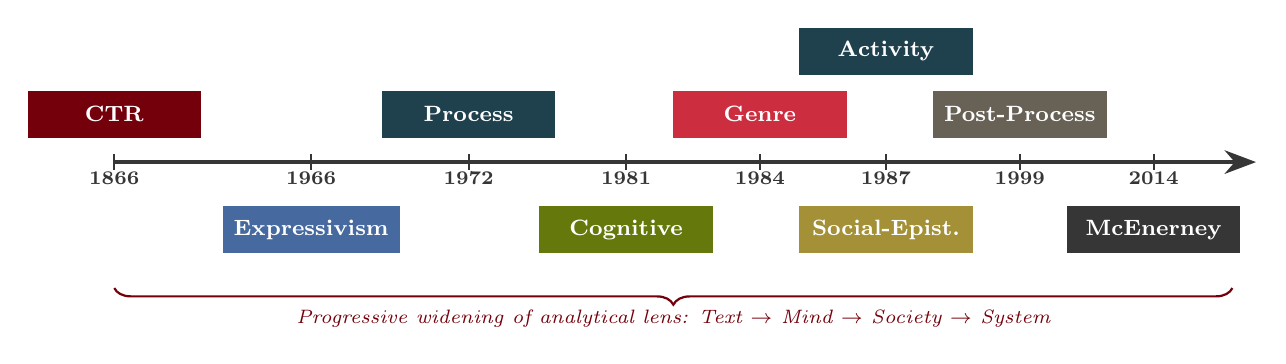
\begin{tikzpicture}[
    every node/.style={font=\footnotesize},
    yearnode/.style={font=\scriptsize\bfseries, text=black90},
    theorybox/.style={rectangle, minimum height=0.6cm, minimum width=2.2cm,
        text=white, font=\footnotesize\bfseries, inner sep=4pt},
]
% Timeline axis
\draw[very thick, black90, -{Stealth[length=4mm]}] (0,0) -- (14.5,0);
\node[yearnode, below] at (0,0) {1866};
\node[yearnode, below] at (2.5,0) {1966};
\node[yearnode, below] at (4.5,0) {1972};
\node[yearnode, below] at (6.5,0) {1981};
\node[yearnode, below] at (8.2,0) {1984};
\node[yearnode, below] at (9.8,0) {1987};
\node[yearnode, below] at (11.5,0) {1999};
\node[yearnode, below] at (13.2,0) {2014};

% Tick marks
\foreach \x in {0,2.5,4.5,6.5,8.2,9.8,11.5,13.2} {
    \draw[thick, black90] (\x,-0.1) -- (\x,0.1);
}

% Theory labels (alternating above/below)
\node[theorybox, fill=garnet, above=0.3cm] at (0,0) {CTR};
\node[theorybox, fill=atlantic, below=0.55cm] at (2.5,0) {Expressivism};
\node[theorybox, fill=congaree, above=0.3cm] at (4.5,0) {Process};
\node[theorybox, fill=horseshoe, below=0.55cm] at (6.5,0) {Cognitive};
\node[theorybox, fill=rose, above=0.3cm] at (8.2,0) {Genre};
\node[theorybox, fill=honeycomb, below=0.55cm] at (9.8,0) {Social-Epist.};
\node[theorybox, fill=warmgrey, above=0.3cm] at (11.5,0) {Post-Process};
\node[theorybox, fill=black90, below=0.55cm] at (13.2,0) {McEnerney};

% Activity Theory overlaps with Social-Epistemic
\node[theorybox, fill=congaree, above=1.1cm] at (9.8,0) {Activity};

% Widening lens annotation
\draw[decorate, decoration={brace, amplitude=6pt, mirror}, thick, garnet]
    (0,-1.6) -- (14.2,-1.6);
\node[font=\scriptsize\itshape, text=garnet, below=0.15cm] at (7.1,-1.6)
    {Progressive widening of analytical lens: Text $\rightarrow$ Mind $\rightarrow$ Society $\rightarrow$ System};

\end{tikzpicture}
\end{document}
